
\section{Semantic Web}
\label{sec:ch2_semantic_web}

In 2001 Tim Berners-Lee, inventor of the World Wide Web and director of World Wide Web Consortium, in his
article published in Scientific American\cite{berneslee:semanticWeb} introduced the term Semantic Web. The
original idea behind this concept is to change the way how WWW works currently, from \lq\lq{}web of
documents\rq\rq{} towards \lq\lq{}web of data\rq\rq{}. The new kind of web will allow machines to
understand the meaning (\emph{semantic}) of information found on the Web. Such an approach will allow
developers to create automated agents that can access Web resources in more intelligent way and thus perform
more complex on user\rq{}s behalf.

From practical point of view, semantic web is all about two things. First, there is need to define common
formats that allows integration and combination of data provided by different, diverse sources. The second big
thing is language that can record how the data relates to real world entities. 

Realization of this idea is currently maintained by Semantic Web
Activity\footnote{\url{http://www.w3.org/2001/sw}} organized within W3C boundaries. This activity with set of
established working groups is responsible for defining technology standards that must be employed in order to
make the Semantic Web operational. Currently, there are following standards defined: RDF, OWL, SPARQL,
RDFa, SKOS, RDFS, GRDDL, POWDER, RIF, SAWSDL. Figure~\ref{fig:sem_web_layers} depicts Semantic Web
\lq\lq{}Layer Cake\rq\rq{} - layers of technologies setting up the concept with layers provided by framework user. Semantic Web responsibility is all above XML (or URI/IRI) and below Unifying Logic components.

\begin{figure}[ht]
  \centering
  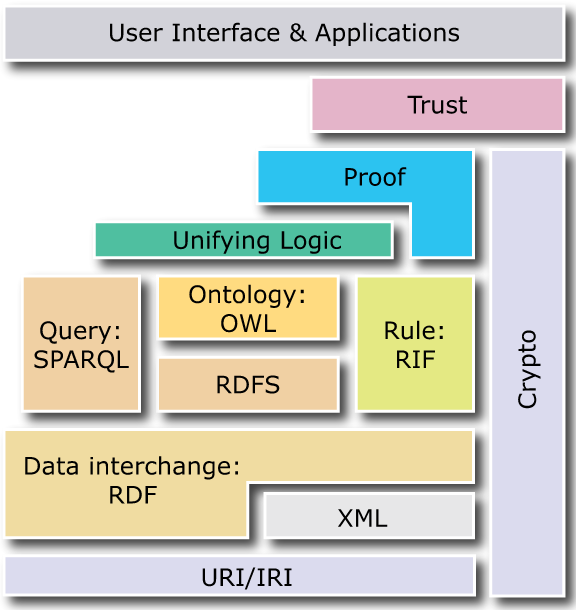
\includegraphics[width=0.6\textwidth]{sem_web_layers}
  \caption{Semantic Web Layer Cake}
  \label{fig:sem_web_layers}
\end{figure}

The following subsections will try to describe roughly most important (in context of this work) of those standards.

\subsection{RDF}

RDF stands for Resource Description Framework (\cite{rdfPrimer:2004}) and it is standard
model for data interchange on the Web. The main idea behind RDF is to make statements about resources. RDF extends the linking structure of the WWW, by adding usage of URIs to name the relationship between entities together with two ends of the link, creating so called \emph{triples} or subject-predicate-object expressions. In this case, subject denotes the resource, predicates demotes traits or aspects of the resource and expresses a relationship between the subject and the object. Using this model standard allows mixing, exposition and sharing of structured and semi-structured data.

This linking structure forms a directed, labeled graph, where the edges represent the named link between
two resources, represented by the graph nodes. Visualization of such a graph forms easiest possible mental model for RDF and is often used in easy-to-understand visual explanations.

In order to make this a bit clearer, let us consider following example. Let us assume, that we\rq{}ve got following statement: \lq\lq{}There is a person called John, whose full name is John Webber, who is British, whose e-mail address is john@agh.edu.pl and is single\rq\rq{} which we would like to represent as RDF graph. Illustration of such a graph can be found in Figure~\ref{fig:sample_rdf}.

\begin{figure}[ht]
  \centering
  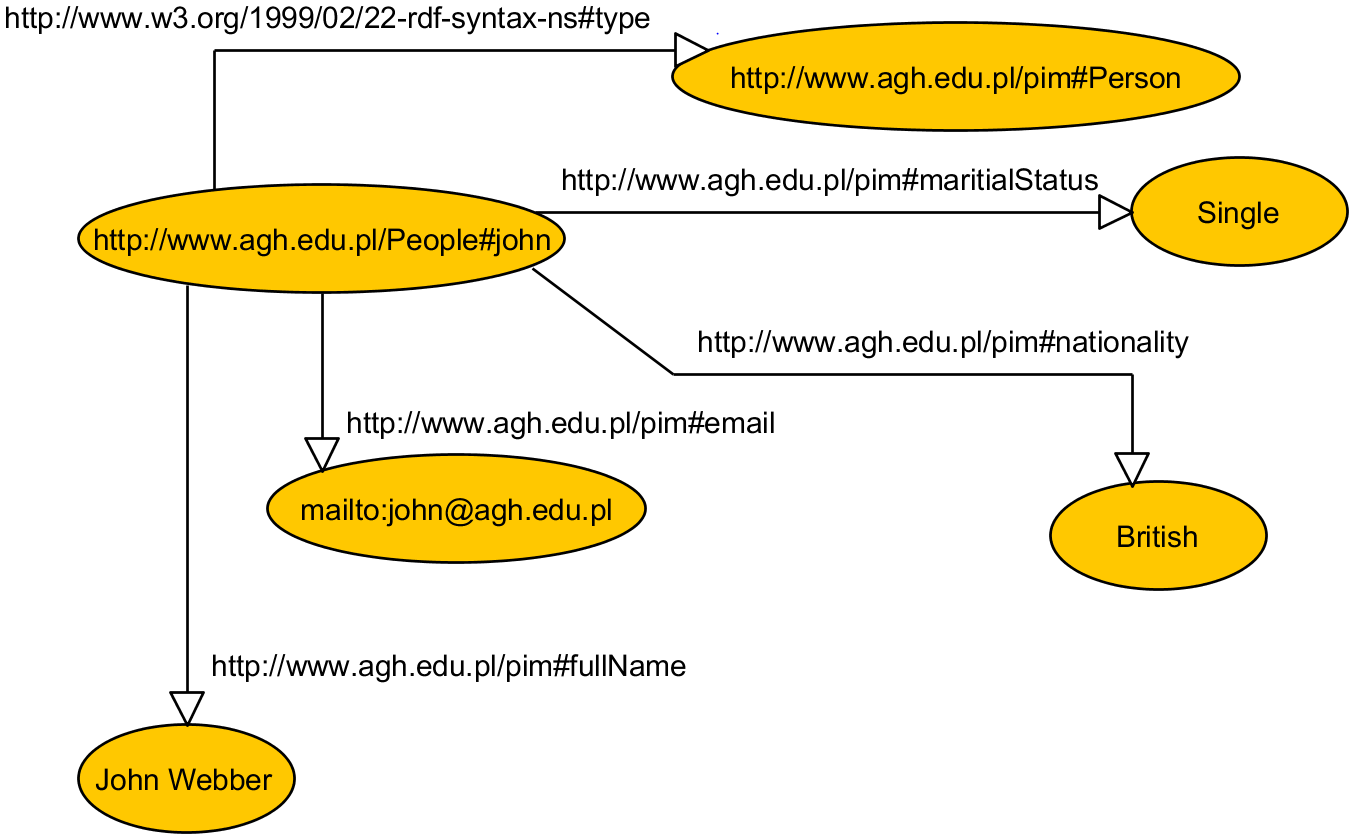
\includegraphics[width=0.8\textwidth]{sample_rdf}
  \caption{RDF Graph representation of example statement.}
  \label{fig:sample_rdf}
\end{figure}

Pure RDF is just a concept, as it\rq{}s name states - framework. In order to actually use this concept, form of data serialization was introduced. RDFS, which stands for RDF Schema\cite{rdfRef:2004}. Most popular form of RDF serialization is using XML (application/rdf+xml mime type). Figure~\ref{fig:whatever} depicts our example using this notation.


\subsection{OWL}

Blah blah\cite{owlRef:2009, owlPrimer:2009}

\subsection{SPARQL}
Blah blah\cite{rdf-sparql-query:2008}
